\chapter{热力学的统计学基础}\label{chap1}

在热物理学的史册中，19世纪50年代是一个极为重要的时代。那时，热力学这门学科——其起源基本上源于对物理系统宏观行为的实验研究——经过卡诺、焦耳、克劳修斯和开尔文等人的不懈努力，已发展成为一门稳固而成熟的物理学分支。热力学前两定律所得出的理论结论，与相应的实验结果呈现出高度一致\footnote{热力学第三定律，也被称为能斯特定理（Nernst's heat theorem），直到1906年左右才出现。关于该定律的一般解释，请参见Simon（1930）和Wilks（1961）；这些参考文献还提供了关于这一主题的广泛参考书目。}。同时，以气体分子运动为基础、试图以微观运动解释宏观性质的气体动理论（kinetic theory of gases），也从更多依赖推测逐步发展为可计算的数学理论。其最初成果可谓卓著；然而直到约 1872 年，玻尔兹曼提出 \(H\) 定理并建立熵与分子动力学的直接联系后，才与热力学实现真正衔接。几乎与此同时，传统动理论也逐步发展为更系统的系综理论（ensemble theory）。最终形成的理论框架把热力学统一为分子力学与统计规律的结果，这一形式自然被称为统计力学（statistical mechanics）。

在为正式理论的建立做准备的过程中，我们首先从一些关于宏观系统统计性质的一般性考量入手。这些考量将为热力学的统计学诠释奠定基础。在此需要指出的是，除非另有说明，所研究的系统应处于其某一平衡状态。

\section{宏观状态与微观状态}\label{section1.1}

我们考虑一个由\(N\)个相同粒子组成的物理系统，这些粒子被限制在体积为\(V\)的空间内。在典型情况下，\(N\)是一个极其庞大的数值——通常约为\(10^{23}\)。鉴于此，人们习惯在所谓的热力学极限（thermodynamic limit）下进行分析，即\(N \to \infty, V \to \infty\)（此时粒子密度 \(n=N/V\) 保持固定）。在这一极限条件下，系统的广延性质（extensive properties）与系统大小成正比（即与\(N\)或\(V\)成正比），而强度性质（intensive properties）与系统大小无关；粒子密度仍是决定系统性质的重要参数。

接下来，我们来考察系统的总能量 \(E\)。如果将构成该系统的粒子视为彼此不相互作用的，则系统的总能量 \(E\) 将等于各单个粒子的能量 \(\varepsilon_i\) 之和：
\begin{equation}\tag{1.2.1}\label{eq:1.2.1}
E = \sum _ { i } n _ { i } \varepsilon _ { i } ,
\end{equation}
其中 \(n_{i}\) 表示每种具有能量 \(\varepsilon_{i}\) 的粒子的数量。显然，
\begin{equation}\tag{1.2.2}\label{eq:1.2.2}
N = \sum _ { i } n _ { i } .
\end{equation}
根据量子力学，单个粒子的能量 \(\varepsilon_{i}\) 是离散的，其取值在很大程度上取决于粒子所受限的体积 \(V\)。因此，总能量 \(E\) 的可能取值也是离散的。然而，当 \(V\) 很大时，不同能量值之间的间隔与系统总能量相比微乎其微，以至于参数 \(E\) 完全可以被视为一个\textbf{连续}变量。即使粒子之间存在相互作用，这种情况依然成立；当然，在这种情况下，总能量 \(E\) 无法以\autoref{eq:1.2.1} 的形式表示。

参数 \(N\)、\(V\) 和 \(E\) 的一个特定取值，对应着给定系统的一个\textbf{宏观状态}（macrostate）。

然而，在分子层面，仍然存在着大量可能性，因为在该尺度上，给定系统的宏观状态 \((N,V,E)\) 可以以多种不同的方式实现。对于非相互作用系统而言，由于总能量 \(E\) 由 \(N\) 个单个粒子的能量 \(\varepsilon_i\) 的简单求和构成，因此显然有大量不同的方式可以选择各自的 \(\varepsilon_i\)，使总能量等于 \(E\)。换句话说，系统总能量 \(E\) 在构成它的 \(N\) 个粒子之间可以被分配出无数种不同的方式。每一种（不同的）方式都定义了给定系统的某一微观状态或微观构型。一般来说，给定系统的各种微观状态或微观构型，可以与该系统的薛定谔方程的独立解 \(\psi(\boldsymbol{r}_1,\ldots,\boldsymbol{r}_N)\) 相对应，这些解对应于相关哈密顿量的特征值 \(E\)。无论如何，给定系统的某一宏观状态通常对应着大量的微观状态；在没有其他约束条件的情况下，人们自然会假设：在任意时刻 \(t\)，系统\textbf{等可能地}处于这些微观状态中的任何一个。这一假设构成了我们理论框架的基石，并通常被称为：对于与给定宏观状态相一致的所有微观状态，均具有``等概率原理''的假说。

当然，所有可能的微观状态的实际数量\(\Omega(N, V, E)\)是\(N\)、\(V\)和\(E\)的函数，其对\(V\)的依赖性源于：单粒子能量的可能取值\(\varepsilon_i\)是\(V\)的函数。令人惊讶的是，正是通过计算\(\Omega\)的大小及其对参数\(N\)、\(V\)和\(E\)的依赖关系，我们才能推导出该系统的完整热力学规律！

我们暂不在此详谈如何计算\(\Omega(N, V, E)\)这个数值；只有在充分发展我们的思考之后，我们才会进一步从该数值出发进行深入推导。首先，我们需要弄清这一数值与各主要热力学量之间的关联方式。为此，我们考虑两个给定物理系统之间的``热接触''问题，希望借助这一思考，揭示\(\Omega\)这一数值的真正本质。

\section{\texorpdfstring{统计学与热力学之间的联系：\(\Omega(N, V, E)\)这一数值的物理意义}{统计学与热力学之间的联系：\textbackslash Omega(N, V, E)这一数值的物理意义}}\label{section1.2}

我们考察两个物理系统\(A_{1}\)和\(A_{2}\)，它们各自处于平衡状态；如图~1.1所示。设\(A_{1}\)的宏观状态由参数\(N_{1}\)、\(V_{1}\)和\(E_{1}\)来表征，因此它拥有\(\Omega_{1}(N_{1}, V_{1}, E_{1})\)个可能的微态；而\(A_{2}\)的宏观状态则由参数\(N_{2}\)、\(V_{2}\)和\(E_{2}\)来表征，因此它拥有\(\Omega_{2}(N_{2}, V_{2}, E_{2})\)个可能的微态。\(\Omega_{1}\)的数学形式未必与\(\Omega_{2}\)的数学形式相同，因为这最终取决于系统的具体性质。当然，我们相信，\(A_{1}\)和\(A_{2}\)这两个系统的所有热力学属性，都可以分别从\(\Omega_{1}(N_{1}, V_{1}, E_{1})\)和\(\Omega_{2}(N_{2}, V_{2}, E_{2})\)这两个函数中推导出来。
现在，我们将这两个系统置于热接触（thermal contact）状态，从而允许两者交换能量；这一过程可通过引入导热壁并移除绝热壁实现。为简化起见，两个系统仍被一堵刚性且不可穿透的壁隔开，因此各自体积\(V_{1}\)和\(V_{2}\)以及粒子数\(N_{1}\)和\(N_{2}\)均保持不变。然而，能量\(E_{1}\)和\(E_{2}\)会随之变化，而限制其变化的唯一条件是
\begin{equation}\tag{1.2.3}\label{eq:1.2.3}
E ^{( 0 )} = E _ { 1 } + E _ { 2 } = \mathrm { c o n s t . }
\end{equation}

\begin{figure}[htbp]
  \centering
  % requires: \usepackage{tikz}
  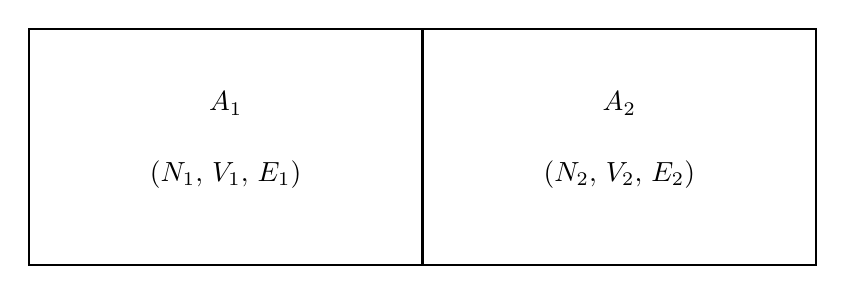
\begin{tikzpicture}[line width=0.8pt]
    % outer rectangle
    \draw (0,0) rectangle (10,3);
    % divider
    \draw (5,0) -- (5,3);

    % left block text
    \node at (2.5,2.05) {$A_{1}$};
    \node at (2.5,1.15) {$(N_{1},\,V_{1},\,E_{1})$};

    % right block text
    \node at (7.5,2.05) {$A_{2}$};
    \node at (7.5,1.15) {$(N_{2},\,V_{2},\,E_{2})$};
  \end{tikzpicture}
  \caption{示意两个系统 \(A_1(N_1,V_1,E_1)\) 与 \(A_2(N_2,V_2,E_2)\) 建立热接触。}
  \label{fig1.1}
\end{figure}



\(^{2}\)值得注意的是，\(\varepsilon_{i}\) 与 \(V\) 的依赖关系本身，是由系统的本质所决定的。例如，相对论系统与非相对论系统的情形并不相同；不妨对比一下第 1.4 节以及问题 1.7 中所讨论的两种情形。此外，我们还应注意到：原则上，\(\Omega\) 与 \(V\) 的依赖关系，源于这样一个事实：正是容器的物理尺寸，体现在对系统波函数施加的边界条件之中。
在此，\(E^{(0)}\) 表示复合系统 \(A^{(0)}\)（即 \(A_{1}+A_{2}\)）的能量；若 \(A_{1}\) 与 \(A_{2}\) 之间存在相互作用能量，则该相互作用能量将被忽略不计。在任意时刻 \(t\)，子系统 \(A_{1}\) 同样有概率处于 \(\Omega_{1}(E_{1})\) 的任一微观态中，而子系统 \(A_{2}\) 同样有概率处于 \(\Omega_{2}(E_{2})\) 的任一微观态中；因此，复合系统 \(A^{(0)}\) 同样有概率处于以下任一状态：
\begin{equation}\tag{1.2.4}\label{eq:1.2.4}
\Omega _ { 1 } ( E _ { 1 } ) \Omega _ { 2 } ( E _ { 2 } ) = \Omega _ { 1 } ( E _ { 1 } ) \Omega _ { 2 } ( E ^{( 0 )} - E _ { 1 } ) = \Omega ^{( 0 )} ( E ^{( 0 )} , E _ { 1 } )
\end{equation}
微观态。\(^{3}\) 显然，\(\Omega^{(0)}\) 本身会随 \(E_{1}\) 的变化而变化。现在的问题是：在何种 \(E_{1}\) 值下，复合系统将达到平衡？换句话说，能量交换需要达到多大程度，才能使子系统 \(A_{1}\) 和 \(A_{2}\) 达到相互平衡？
我们断言，这一过程将在 \(E_{1}\) 取得最大值时发生——即 \(\Omega^{(0)}(E^{(0)},E_{1})\) 的最大值所在处。其背后的哲学思想是：当一个物理系统被置于自然状态时，它会自然而然地朝向这样一种方向发展：通过不断增加微观态的数量，直至最终稳定于一个宏观态，而这个宏观态恰好拥有最多数量的微观态。从统计学的角度来看，我们认为，具有更多微观态的宏观态更为可能，而拥有最多微观态的宏观态则被视为最可能的状态。详细研究表明，对于典型的系统而言，任何偏离最可能宏观态的微观态数量，都比后者少上"数量级"之多。因此，系统的最可能状态，就是那个系统在其中度过"绝大多数"时间的宏观态。由此，将这一状态等同于系统的平衡状态，也就显得顺理成章。
我们将 \(E_{1}\) 的平衡值记作 \(\overline{E}_{1}\)（\(E_{2}\) 的平衡值记作 \(\overline{E}_{2}\)），在最大化 \(\Omega^{(0)}\) 时，我们得到：
\begin{equation}\tag{1.2.5}\label{eq:1.2.5}
\left( \frac { \partial \Omega _ { 1 } ( E _ { 1 } ) } { \partial E _ { 1 } } \right) _ { E _ { 1 } = \overline { { E } } _ { 1 } } \Omega _ { 2 } ( \overline { { E } } _ { 2 } ) + \Omega _ { 1 } ( \overline { { E } } _ { 1 } ) \left( \frac { \partial \Omega _ { 2 } ( E _ { 2 } ) } { \partial E _ { 2 } } \right) _ { E _ { 2 } = \overline { { E } } _ { 2 } } \cdot \frac { \partial E _ { 2 } } { \partial E _ { 1 } } = 0 .
\end{equation}
由于 \(\partial E_{2}/\partial E_{1}=-1\)，详见\autoref{eq:1.3.1}，上述条件可写为
\begin{equation}\tag{1.2.6}\label{eq:1.2.6}
\left( \frac { \partial \ln \Omega _ { 1 } ( E _ { 1 } ) } { \partial E _ { 1 } } \right) _ { E _ { 1 } = \overline { { E } } _ { 1 } } = \left( \frac { \partial \ln \Omega _ { 2 } ( E _ { 2 } ) } { \partial E _ { 2 } } \right) _ { E _ { 2 } = \overline { { E } } _ { 2 } } .
\end{equation}
因此，我们关于平衡状态的条件归结为子系统 \(A_{1}\) 和 \(A_{2}\) 分别的参数 \(\beta_{1}\) 和 \(\beta_{2}\) 的相等。其中，\(\beta\) 的定义如下：
\begin{equation}\tag{1.2.7}\label{eq:1.2.7}
\beta \equiv \left( \frac { \partial \ln \Omega ( N , V , E ) } { \partial E } \right) _ { N , V , E = \overline { { E } } } .
\end{equation}
³ 显而易见，复合系统 \(A^{(0)}\) 的宏观状态必须由两种能量来确定，即 \(E_{1}\) 和 \(E_{2}\)（否则，就只能是 \(E^{(0)}\) 与 \(E_{1}\)）。
因此，我们发现，当两个物理系统相互接触并实现能量交换时，这种能量交换会持续进行，直到变量 \(E_{1}\) 和 \(E_{2}\) 的平衡值 \(\overline{E}_{1}\) 和 \(\overline{E}_{2}\) 被达到。一旦这两个值被达到，两个系统之间便不再有净能量交换；此时，人们称这两个系统已达到热平衡状态。根据我们的分析，只有当参数 \(\beta\) 的相应值——即 \(\beta_{1}\) 和 \(\beta_{2}\)——相等时，这一过程才会发生。⁴ 因此，我们自然会预期，参数 \(\beta\) 与某一特定系统的热力学温度 \(T\) 存在某种关联。为了确定这一关系，我们回顾热力学公式
\begin{equation}\tag{1.2.8}\label{eq:1.2.8}
\left( \frac { \partial S } { \partial E } \right) _ { N , V } = \frac { 1 } { T } ,
\end{equation}
其中 \(S\) 为该系统的熵。将\autoref{eq:1.3.3} 与\autoref{eq:1.3.4} 进行比较，我们得出结论：热力学量 \(S\) 与统计量 \(\Omega\) 之间存在着密切的联系；事实上，对于任意一个物理系统，我们都可以写成
\begin{equation}\tag{1.2.9}\label{eq:1.2.9}
{ \frac { \Delta S } { \Delta ( \ln \Omega ) } } = { \frac { 1 } { \beta T } } = \mathrm { c o n s t . }
\end{equation}
这一对应关系最早由玻尔兹曼确立，他同时认为，由于热力学方法与统计学方法之间的关系似乎具有根本性，因此\autoref{eq:1.3.5} 中出现的常数必然是一个普遍常数。正是普朗克首次给出了明确的公式
\begin{equation}\tag{1.2.10}\label{eq:1.2.10}
S = k \ln \Omega ,
\end{equation}
不包含任何附加常数 \(S_0\)。目前，\autoref{eq:1.3.6} 以总微态数量为依据，根据给定的宏观状态，确定了某一特定物理系统的熵的绝对值。熵的零点则对应于一种特殊的状态，在这种状态下，仅有一个微态可被访问（\(\Omega=1\)）——即所谓的"唯一构型"；因此，统计学方法也为热力学第三定律提供了理论基础。\autoref{eq:1.3.6} 在物理学中具有至关重要的意义，它架起了微观世界与宏观世界之间的桥梁。
在热力学第二定律的研究中，我们了解到，熵增原理与这样一个事实密切相关：在宇宙的自然演化过程中，宇宙中的能量含量正日益减少，而可供转化为功的能量也越来越少；因此，某一特定系统的熵可以被视为衡量该系统中所普遍存在的"无序"或"混乱"的一种指标。公式（6）向我们揭示了无序是如何在微观层面产生的。显然，无序正是系统所能存在微态数量之多的体现。微态的选择越多，系统的可预测性就越低，从而导致系统中无序程度的升高。当系统完全处于有序状态时，
只有当系统别无选择，只能处于唯一一个状态（\(\Omega = 1\)）时，这一状态才对应于熵为零的状态。
根据公式（5）和（6），我们还得到
\begin{equation}\tag{1.2.11}\label{eq:1.2.11}
\beta = { \frac { 1 } { k T } } .
\end{equation}
普遍常数 \(k\) 通常被称为玻尔兹曼常数。在第1.4节中，我们将进一步探究 \(k\) 与气体常数 \(R\) 和阿伏伽德罗常数 \(N_{A}\) 之间的关系；详见公式（1.4.3）。\(^{5}\)
1.3 统计学与热力学的进一步联系
在延续前文的讨论之后，我们现在来探讨子系统 \(A_{1}\) 与 \(A_{2}\) 之间更为复杂的相互作用。若假设分隔两个子系统的壁既可移动又具有导电性，那么子系统 \(A_{1}\) 和 \(A_{2}\) 的各自体积 \(V_{1}\) 和 \(V_{2}\) 也会随之发生变化；事实上，总体积 \(V^{(0)}\)（即 \(V_{1}+V_{2}\)）保持不变，因此实际上我们只多出一个独立变量。当然，我们仍假定该壁对粒子完全不透，因此 \(N_{1}\) 和 \(N_{2}\) 的数值依然固定。按照先前的论证，当子系统 \(A^{(0)}\) 的状态熵 \(\Omega^{(0)}(V^{(0)},E^{(0)};V_{1},E_{1})\) 达到最大值时，复合系统 \(A^{(0)}\) 将达到平衡状态；也就是说，不仅
\begin{equation}\tag{1.3.1}\label{eq:1.3.1}
\left( \frac { \partial \ln \Omega _ { 1 } } { \partial E _ { 1 } } \right) _ { N _ { 1 } , V _ { 1 } ; \, E _ { 1 } = \overline { { E } } _ { 1 } } = \left( \frac { \partial \ln \Omega _ { 2 } } { \partial E _ { 2 } } \right) _ { N _ { 2 } , V _ { 2 } ; \, E _ { 2 } = \overline { { E } } _ { 2 } } ,
\end{equation}
而且
\begin{equation}\tag{1.3.2}\label{eq:1.3.2}
\left( \frac { \partial \ln \Omega _ { 1 } } { \partial V _ { 1 } } \right) _ { N _ { 1 } , E _ { 1 } ; \; V _ { 1 } = \overline { { V } } _ { 1 } } = \left( \frac { \partial \ln \Omega _ { 2 } } { \partial V _ { 2 } } \right) _ { N _ { 2 } , E _ { 2 } ; \; V _ { 2 } = \overline { { V } } _ { 2 } } .
\end{equation}
我们关于平衡状态的条件现在表现为：子系统 \(A_{1}\) 的参数对 \((\beta_{1},\eta_{1})\) 与子系统 \(A_{2}\) 的参数对 \((\beta_{2},\eta_{2})\) 之间满足等式，而根据定义，
\begin{equation}\tag{1.3.3}\label{eq:1.3.3}
\eta \equiv \left( \frac { \partial \ln \Omega ( N , V , E ) } { \partial V } \right) _ { N , E , V = \overline { { V } } } .
\end{equation}
同样地，如果 \(A_{1}\) 和 \(A_{2}\) 通过一堵允许粒子交换的壁彼此接触，那么平衡状态的条件还将因以下等式而进一步加强：
子系统 \(A_{1}\) 的参数 \(\zeta_{1}\) 与子系统 \(A_{2}\) 的参数 \(\zeta_{2}\) 之间也满足等式，而根据定义，
\begin{equation}\tag{1.3.4}\label{eq:1.3.4}
\zeta \equiv \left( \frac { \partial \ln \Omega ( N , V , E ) } { \partial N } \right) _ { V , E , N = \overline { { { N } } } } .
\end{equation}
为了确定参数 \(\eta\) 和 \(\zeta\) 的物理意义，我们借助\autoref{eq:1.2.6} 以及热力学的基本公式，即
\begin{equation}\tag{1.3.5}\label{eq:1.3.5}
d E = T \, d S - P \, d V + \mu \, d N ,
\end{equation}
其中 \(P\) 为热力学压力，\(\mu\) 为给定体系的化学势。由此可得
\begin{equation}\tag{1.3.6}\label{eq:1.3.6}
\eta = \frac { P } { k T }  \mathrm { a n d }  \zeta = - \frac { \mu } { k T } .
\end{equation}
从物理角度来看，这些结果完全令人满意，因为在热力学意义上，当两个系统 \(A_{1}\) 和 \(A_{2}\) 之间处于平衡状态时，若将二者隔开的壁既具有导电性又可移动（从而使其各自的能量和体积发生变化），那么其条件与\autoref{eq:1.3.1} 和 \autoref{eq:1.3.1} 中所包含的条件实际上完全一致，即
\begin{equation}\tag{1.3.7}\label{eq:1.3.7}
T _ { 1 } = T _ { 2 }  \mathrm { a n d }  P _ { 1 } = P _ { 2 } .
\end{equation}
另一方面，如果这两个系统既能交换粒子，又能交换能量，但其体积保持固定，那么在热力学上所获得的平衡条件，确实为
\begin{equation}\tag{1.3.8}\label{eq:1.3.8}
T _ { 1 } = T _ { 2 }  \mathrm { a n d }  \mu _ { 1 } = \mu _ { 2 } .
\end{equation}
最后，若交换过程使得这三种（宏观）参数均变为可变，则平衡条件将变为
\begin{equation}\tag{1.3.9}\label{eq:1.3.9}
T _ { 1 } = T _ { 2 } ,  P _ { 1 } = P _ { 2 } ,  \mathrm { a n d }  \mu _ { 1 } = \mu _ { 2 } .
\end{equation}
令人欣慰的是，这些结论与基于统计学考量所得出的结果完全一致。
结合前述讨论的结果，我们得出以下从统计学出发推导热力学的法则：对于给定系统的宏观态 \((N,V,E)\)，确定该系统所能达到的所有可能微观态的数量；将这一数量称为 \(\Omega(N,V,E)\)。随后，该状态下系统的熵可由
基本公式
\begin{equation}\tag{1.3.10}\label{eq:1.3.10}
S ( N , V , E ) = k \ln \Omega ( N , V , E ) ,
\end{equation}
而主导的强度场——即温度、压力和化学势——则由
\begin{equation}\tag{1.3.11}\label{eq:1.3.11}
\left( \frac { \partial S } { \partial E } \right) _ { N , V } = \frac { 1 } { T } ;  \left( \frac { \partial S } { \partial V } \right) _ { N , E } = \frac { P } { T } ;  \left( \frac { \partial S } { \partial N } \right) _ { V , E } = - \frac { \mu } { T } .
\end{equation}
或者，我们也可以写成
\begin{equation}\tag{1.3.12}\label{eq:1.3.12}
P = \left( \frac { \partial S } { \partial V } \right) _ { N , E } \Bigg / \left( \frac { \partial S } { \partial E } \right) _ { N , V } = - \left( \frac { \partial E } { \partial V } \right) _ { N , S }
\end{equation}
以及
\begin{equation}\tag{1.3.13}\label{eq:1.3.13}
\mu = - \left( \frac { \partial S } { \partial N } \right) _ { V , E } \bigg / \left( \frac { \partial S } { \partial E } \right) _ { N , V } = \left( \frac { \partial E } { \partial N } \right) _ { V , S } ,
\end{equation}
同时，
\begin{equation}\tag{1.3.14}\label{eq:1.3.14}
T = \left( { \frac { \partial E } { \partial S } } \right) _ { N , V } .
\end{equation}
\autoref{eq:1.3.11} 至 \autoref{eq:1.3.13} 也同样可以由\autoref{eq:1.3.4} 得到。事实上，要根据这些公式计算 \(P\)、\(\mu\) 和 \(T\)，必须将能量 \(E\) 表示为 \(N\)、\(V\) 和 \(S\) 的函数；原则上，一旦 \(S\) 被知悉为 \(N\)、\(V\) 和 \(E\) 的函数，这一操作便应成为可能。
其余的热力学内容则可轻松推导出来；请参阅附录 H。例如，亥姆霍兹自由能 \(A\)、吉布斯自由能 \(G\) 以及焓 \(H\) 分别由
\begin{equation}\tag{1.3.15}\label{eq:1.3.15}
\begin{array}{rl} & { A = E - T S , } \\& { G = A + P V = E - T S + P V } \\& { = \mu N } \end{array}
\end{equation}
\(^{7}\)在撰写这些公式时，我们运用了偏微分学中广为人知的关系，即"若三个变量 \(x\)、\(y\) 和 \(z\) 之间存在相互关系，则（参见附录 H）
\begin{equation}\tag{1.3.16}\label{eq:1.3.16}
\left(\frac{\partial x}{\partial y}\right)_z\left(\frac{\partial y}{\partial z}\right)_x\left(\frac{\partial z}{\partial x}\right)_y=-1."
\end{equation}
\(^{8}\)关系 \(E-TS+PV=\mu N\) 可以直接从式（4）中推导出来。为此，我们只需将所给系统视为在渐进的过程中逐渐扩展至当前尺寸，使得在这一过程中，各组分参数 \(T\)、\(P\) 和 \(\mu\) 保持恒定，而广延参数 \(N\)、\(V\) 和 \(E\)（以及由此产生的 \(S\)）则彼此按比例相应地增长。
并且
\begin{equation}\tag{1.3.17}\label{eq:1.3.17}
H = E + P V = G + T S .
\end{equation}
定容热容 \(C_{V}\) 与定压热容 \(C_{P}\) 分别为：
\begin{equation}\tag{1.3.18}\label{eq:1.3.18}
C _ { V } \equiv T \left( \frac { \partial S } { \partial T } \right) _ { N , V } = \left( \frac { \partial E } { \partial T } \right) _ { N , V }
\end{equation}
并且
\begin{equation}\tag{1.3.19}\label{eq:1.3.19}
C _ { P } \equiv T \left( \frac { \partial S } { \partial T } \right) _ { N , P } = \left( \frac { \partial ( E + P V ) } { \partial T } \right) _ { N , P } = \left( \frac { \partial H } { \partial T } \right) _ { N , P } .
\end{equation}
\section{经典理想气体}\label{ux7ecfux5178ux7406ux60f3ux6c14ux4f53}
为了说明前几节所阐述的分析方法，我们现在将推导出由单原子分子构成的经典理想气体的各项热力学性质。我们之所以选择这一高度专业化的体系进行研究，主要是因为它能够对数 \(\Omega(N,V,E)\) 进行明确且近乎渐近式的计算。当我们发现通过研究这一体系，我们可以以最直观的方式，借助其他物理常数来确定玻尔兹曼常数 \(k\)——详见式（3）——这一事实更加凸显了其重要性。此外，该体系的行为也为研究其他物理系统提供了有益的参考依据，尤其是那些真实气体（无论是否受到量子效应的影响）。事实上，在高温低密度的极限条件下，理想气体的行为便成为大多数真实系统的典型行为。
在对这一案例展开详细研究之前，有必要先指出一点，这一点适用于所有由非相互作用粒子构成的经典系统，无论这些粒子的内部结构如何。这一要点与数 \(\Omega(N,V,E)\) 对 \(V\) 的显式依赖性有关，进而也与这些系统的状态方程息息相关。如果粒子之间不存在任何空间上的相关性，也就是说，任何一个粒子出现在可用空间特定区域的概率完全独立于其他粒子的位置，那么 \(N\) 个粒子在系统中进行空间分布的总方式数，将仅仅等于各个粒子在各自独立的空间中占据位置的方式数的乘积。在 \(N\) 和 \(E\) 固定的情况下，这两个数值将与容器的体积 \(V\) 成正比；相应地，总方式数也将与 \(V\) 的 \(N\) 次方成正比：
\begin{equation}\tag{1.3.20}\label{eq:1.3.20}
\Omega ( N , E , V ) \propto V ^{N} .
\end{equation}
若满足以下两个条件，则上述结论成立：（1）粒子之间的相互作用可以忽略不计；（2）单个粒子的波包不会发生显著重叠——换言之，量子效应同样可以忽略不计。
结合方程（1.3.9）和（1.3.10），我们得到
\begin{equation}\tag{1.3.21}\label{eq:1.3.21}
\frac { P } { T } = k \left( \frac { \partial \ln \Omega ( N , E , V ) } { \partial V } \right) _ { N , E } = k \frac { N } { V } .
\end{equation}
若系统中包含 \(n\) 摩尔的气体，则 \(N = nN_A\)，其中 \(N_A\) 是阿伏伽德罗常数。于是，方程（2）变为
\begin{equation}\tag{1.3.22}\label{eq:1.3.22}
P V = N k T = n R T  ( R = k N _ { A } ) ,
\end{equation}
这就是著名的理想气体状态方程，其中 \(R\) 为每摩尔气体的气体常数。因此，对于任何由非相互作用粒子组成的经典系统而言，理想气体状态方程均适用。
要推导该系统的其他热力学性质，我们需要深入了解 \(\Omega\) 如何依赖于参数 \(N\)、\(V\) 和 \(E\)。问题本质上归结为：确定方程（1.1.1）和（1.1.2）同时满足的总方式数。换句话说，我们必须计算出满足方程的总方式数（即独立的方式数）。
\begin{equation}\tag{1.3.23}\label{eq:1.3.23}
\sum _ { r = 1 } ^{3 N} \varepsilon _ { r } = E ,
\end{equation}
其中 \(\varepsilon_{r}\) 分别对应 \(N\) 个粒子各自由度所对应的能量。之所以这一数值需要依赖于参数 \(N\) 和 \(E\)，原因十分显而易见。然而，这一数值同样取决于变量 \(\varepsilon_{r}\) 可取的"值域"；正是通过这一值域，才产生了对 \(V\) 的依赖关系。现在，对于一个自由的、非相对论性粒子，其能量本应满足以下条件：该粒子被限制在边长为 \(L\) 的立方体盒中（\(V=L^{3}\)），且波函数 \(\psi(\boldsymbol{r})\) 在边界上处处为零。此时，该粒子的能量本应满足以下公式：
\begin{equation}\tag{1.3.24}\label{eq:1.3.24}
\varepsilon ( n _ { x } , n _ { y } , n _ { z } ) = \frac { h ^{2} } { 8 m L ^{2} } ( n _ { x } ^{2} + n _ { y } ^{2} + n _ { z } ^{2} ) ;  n _ { x } , n _ { y } , n _ { z } = 1 , 2 , 3 , \ldots ,
\end{equation}
其中 \(h\) 是普朗克常数，\(m\) 是粒子的质量。因此，对于能量为 \(\varepsilon\) 的粒子，其不同的本征函数（或微态）的数量，将等于方程
\begin{equation}\tag{1.3.25}\label{eq:1.3.25}
\left( n _ { x } ^{2} + n _ { y } ^{2} + n _ { z } ^{2} \right) = \frac { 8 m V ^{2 / 3} \varepsilon } { \hbar ^{2} } = \varepsilon ^{*} .
\end{equation}
我们可以将这一数量记作 \(\Omega(1,\varepsilon,V)\)。进一步推演可知，所求的总数 \(\Omega(N,E,V)\) 将等于方程
\begin{equation}\tag{1.3.26}\label{eq:1.3.26}
\sum _ { r = 1 } ^{3 N} n _ { r } ^{2} = \frac { 8 m V ^{2 / 3} E } { h ^{2} } = E ^{*} ,  \mathrm { s a y } .
\end{equation}
从方程（7）中可直接得出一个重要结论，甚至在明确计算出 \(\Omega(N,E,V)\) 之前即可得出。根据该方程右侧表达式的本质，我们推断：系统的体积 \(V\) 和能量 \(E\) 以 \((V^{2/3}E)\) 这一组合的形式，纳入了 \(\Omega\) 的表达式之中。因此，
\begin{equation}\tag{1.3.27}\label{eq:1.3.27}
S ( N , V , E ) \equiv S \Bigl ( N , V ^{2 / 3} E \Bigr ) .
\end{equation}
由此可见，为了使 \(S\) 和 \(N\) 保持恒定，从而定义一个可逆绝热过程，
\begin{equation}\tag{1.3.28}\label{eq:1.3.28}
V ^{2 / 3} E = \mathrm { c o n s t . }
\end{equation}
方程（1.3.11）由此得出
\begin{equation}\tag{1.3.29}\label{eq:1.3.29}
P = - \left( { \frac { \partial E } { \partial V } } \right) _ { N , S } = { \frac { 2 } { 3 } } { \frac { E } { V } } ,
\end{equation}
也就是说，非相对论性、非相互作用粒子系统的压力恰好等于其能量密度的三分之二。\(^{10}\) 值得注意的是，由于尚未对数 \(\Omega\) 进行明确的计算，因此结果（9）和（10）既适用于量子统计，也适用于经典统计；将这两者结合起来所得的结果同样具有普遍性，即
\begin{equation}\tag{1.3.30}\label{eq:1.3.30}
P V ^{5 / 3} = \mathrm { c o n s t . } ,
\end{equation}
这告诉我们，在可逆绝热过程中，\(P\) 如何随 \(V\) 变化。
接下来，我们将尝试对数 \(\Omega\) 进行求值。在这一求值过程中，我们明确假设粒子是可区分的，因此，如果状态 \(i\) 中的某个粒子与状态 \(j\) 中的某个粒子发生互换，则所得到的微观状态将被计为不同的状态。因此，数 \(\Omega(N,V,E)\)，或者更准确地说，\(\Omega_{N}(E^{*})\)（参见式（7）），等于位于一个 \(3N\) 维球面上、半径为 \(\sqrt{E^{*}}\) 的正整数点的数量。显然，这个数会随着 \(E^{*}\) 的变化呈现出极其不规则的特性：对于两个给定的 \(E^{*}\) 值，尽管它们可能彼此非常接近，但该数的取值却可能大相径庭。相比之下，数 \(\Sigma_{N}(E^{*})\)——即位于或位于以 \(\sqrt{E^{*}}\) 为半径的 \(3N\) 维球面表面或其内部的正整数点数量——则要不那么不规则。就我们的物理问题而言，这相当于系统中微态的数量 \(\Sigma(N,V,E)\)，即在满足所有由参数 \(N\) 和 \(V\) 确定的宏观状态的前提下，且能量低于
大于或等于 \(E\)；也就是说，
\begin{equation}\tag{1.3.31}\label{eq:1.3.31}
\Sigma ( N , V , E ) = \sum _ { E ^{\prime} \leq E } \Omega ( N , V , E ^{\prime} )
\end{equation}
或者
\begin{equation}\tag{1.3.32}\label{eq:1.3.32}
\sum _ { N } ( E ^{*} ) = \sum _ { E ^{* ^ { \prime} } \leq E ^{*} } \Omega _ { N } ( E ^{* ^ { \prime} } ) .
\end{equation}
当然，数 \(\Sigma\) 也会存在一定程度的不规则性；然而，我们预期，当 \(E^{*} \rightarrow \infty\) 时，它的渐近行为将比 \(\Omega\) 的渐近行为平滑得多。在后续的讨论中，我们将看到，该系统的热力学性质，无论是从数 \(\Sigma\) 还是从数 \(\Omega\) 得到的，都同样能够很好地描述。
要理解此处所阐述的观点，不妨稍作离题，深入探讨数值 \(\Omega_{1}(\varepsilon^{*})\) 和 \(\Sigma_{1}(\varepsilon^{*})\) 的行为——这两者对应于单个粒子被限制在给定体积 \(V\) 中的情形。对于 \(\varepsilon^{*} \leq 10,000\)，这些数值的精确取值可从古普塔（1947）编撰的表格中获得。数值 \(\Omega_{1}(\varepsilon^{*})\) 那些剧烈而不规则的变化几乎难以忽视。相比之下，数值 \(\Sigma_{1}(\varepsilon^{*})\) 则呈现出更为平滑的渐近行为。从问题的几何结构出发，我们注意到：在渐近意义上，\(\Sigma_{1}(\varepsilon^{*})\) 应当等于一个半径为 \(\sqrt{\varepsilon^{*}}\) 的三维球体中一个八分之一象限的体积，即，
\begin{equation}\tag{1.3.33}\label{eq:1.3.33}
\operatorname* { l i m } _ { \varepsilon ^{*} \to \infty } { \frac { \sum _ { 1 } ( \varepsilon ^{*} ) } { ( \pi / 6 ) \varepsilon ^{* 3 / 2} } } = 1 .
\end{equation}
更细致的分析表明，按照下一次近似计算（参见帕特里亚，1966），
\begin{equation}\tag{1.3.34}\label{eq:1.3.34}
\Sigma _ { 1 } ( \varepsilon ^{*} ) \approx \frac { \pi } { 6 } \varepsilon ^{* 3 / 2} - \frac { 3 \pi } { 8 } \varepsilon ^{*} ;
\end{equation}
修正项的产生源于这样一个事实：八分之一象限的体积在一定程度上高估了所需晶格点的数量，因为它在某种程度上包含了那些某个或多个坐标为零的点。图~1.2展示了 \(\varepsilon^{*}\) 介于200至300之间的 \(\Sigma_{1}(\varepsilon^{*})\) 实际数值的直方图；同时，也展示了理论估算值（15）。在图中，我们还加入了相应微态数量 \(\Sigma_{1}^{\prime}(\varepsilon^{*})\) 的实际数值直方图——当量子数 \(n_{x}\)、\(n_{y}\) 和 \(n_{z}\) 均可取零值时的情况。在后一种情况下，八分之一象限的体积在一定程度上低估了所需晶格点的数量；如今，我们得到了
\begin{equation}\tag{1.3.35}\label{eq:1.3.35}
\Sigma _ { 1 } ^{\prime} ( \varepsilon ^{*} ) \approx \frac { \pi } { 6 } \varepsilon ^{* 3 / 2} + \frac { 3 \pi } { 8 } \varepsilon ^{*} .
\end{equation}
然而，在渐近意义上，数值 \(\Sigma_{1}^{\prime}(\varepsilon^{*})\) 也满足方程（14）。
回到 \(N\) 个粒子的问题，数值 \(\Sigma_{N}(E^{*})\) 在渐近意义上应等于一个 \(3N\) 维球体中"正向区域"的"体积"。
对数运算并应用斯特林公式（附录~B中的方程B.29），
\begin{equation}\tag{1.3.36}\label{eq:1.3.36}
\ln ( n ! ) \approx n \ln n - n  ( n \gg 1 ) ,
\end{equation}
我们得到
\begin{equation}\tag{1.3.37}\label{eq:1.3.37}
\ln \Sigma ( N , V , E ) \approx N \ln \left[ \frac { V } { h ^{3} } \left( \frac { 4 \pi m E } { 3 N } \right) ^{3 / 2} \right] + \frac { 3 } { 2 } N .
\end{equation}
要推导所给系统的热力学性质，我们不得不以某种方式确定系统的能量的精确值，或为其设定一个限定范围。鉴于函数 \(\Omega(N,V,E)\) 的特性极其不规则，从物理角度而言，无法为系统的能量赋予一个确切的数值，因为这样无论如何都无法得到系统热力学函数的光滑、连续的表达式。从实际应用的角度来看，完全孤立的系统也过于理想化。在现实世界中，几乎每一个系统都会与周围环境存在一定的相互作用，哪怕这种相互作用微乎其微；因此，系统的能量无法被精确地界定。¹² 当然，能量变化范围的实际宽度，与能量的平均值相比，通常都相当小。我们不妨将这一范围限定为 \(E - \frac{1}{2}\Delta\) 和 \(E + \frac{1}{2}\Delta\) 两个极限值——假设 \(\Delta \ll E\)；通常情况下，\(\Delta/E = O(1/\sqrt{N})\)。相应地，系统的微观状态数 \(\Gamma(N,V,E;\Delta)\) 可以表示为：
\begin{equation}\tag{1.3.38}\label{eq:1.3.38}
\Gamma ( N , V , E ; \Delta ) \simeq \frac { \partial \Sigma ( N , V , E ) } { \partial E } \Delta \approx \frac { 3 N } { 2 } \frac { \Delta } { E } \Sigma ( N , V , E ) ,
\end{equation}
由此可得
\begin{equation}\tag{1.3.39}\label{eq:1.3.39}
\ln \Gamma ( N , V , E ; \Delta ) \approx N \ln \left[ \frac { V } { \hbar ^{3} } \left( \frac { 4 \pi m E } { 3 N } \right) ^{3 / 2} \right] + \frac { 3 } { 2 } N + \left\{ \ln \left( \frac { 3 N } { 2 } \right) + \ln \left( \frac { \Delta } { E } \right) \right\} .
\end{equation}
现在，当 \(N \gg 1\) 时，花括号中的第一项与括号外的任何项相比都可忽略不计，因为 \(\lim_{N \to \infty} (\ln N)/N = 0\)。此外，对于任意合理的 \(\Delta/E\) 值，花括号中的第二项也同样如此。¹³ 因此，在实际应用中，
\begin{equation}\tag{1.3.40}\label{eq:1.3.40}
\ln \Gamma \approx \ln \Sigma \approx \mathcal { N } \ln \left[ \frac { V } { \hbar ^{3} } \left( \frac { 4 \pi m E } { 3 N } \right) ^{3 / 2} \right] + \frac { 3 } { 2 } N .
\end{equation}
于是，我们得到了一个令人费解的结果：在实际应用中，系统能量允许变化的范围实际上差异不大；能量可能介于 \(E - \frac{1}{2}\Delta\) 与 \(E + \frac{1}{2}\Delta\) 之间，或者同样可以是 0 与 \(E\) 之间。造成这一现象的原因在于，系统微观状态数的增长速率
随着能量的增加而呈指数级增长，这一点在式（1.4.17） 中已有充分说明；即使我们允许能量取任意介于 0 与某一特定值 \(E\) 之间的数值，真正对这一数量贡献最大的，也仅仅是 \(E\) 的"近邻区域"！而且，由于我们最终只关心这一数量的对数，因此即便只是该"近邻区域"的"宽度"，也已不再具有重要意义！
如今，我们已经为推导系统的热力学性质做好了充分准备。首先，我们有
\begin{equation}\tag{1.3.41}\label{eq:1.3.41}
S ( N , V , E ) = k \ln \Gamma = N k \ln \left[ \frac { V } { \hbar ^{3} } \left( \frac { 4 \pi \, m E } { 3 N } \right) ^{3 / 2} \right] + \frac { 3 } { 2 } N k ,
\end{equation}
该式可逆代换，从而得到
\begin{equation}\tag{1.3.42}\label{eq:1.3.42}
E ( S , V , N ) = \frac { 3 h ^{2} N } { 4 \pi m V ^{2 / 3} } \exp \left( \frac { 2 S } { 3 N k } - 1 \right) .
\end{equation}
随后，借助\autoref{eq:1.3.10} 或 \autoref{eq:1.3.13}，即可求得气体的温度，并由此得出能量与温度的关系式
\begin{equation}\tag{1.3.43}\label{eq:1.3.43}
E = N \bigg ( \frac { 3 } { 2 } k T \bigg ) = n \bigg ( \frac { 3 } { 2 } R T \bigg ) ,
\end{equation}
其中，\(n\) 为气体的摩尔数。借助公式（1.3.17），可得恒容热容：
\begin{equation}\tag{1.3.44}\label{eq:1.3.44}
C _ { V } = \left( \frac { \partial E } { \partial T } \right) _ { N , V } = \frac { 3 } { 2 } N k = \frac { 3 } { 2 } n R .
\end{equation}
对于状态方程，我们得到
\begin{equation}\tag{1.3.45}\label{eq:1.3.45}
P = - \left( \frac { \partial E } { \partial V } \right) _ { N , S } = \frac { 2 } { 3 } \frac { E } { V } ,
\end{equation}
这一结果与我们先前得出的结论（10）一致。结合（23），我们得到
\begin{equation}\tag{1.3.46}\label{eq:1.3.46}
P = { \frac { N k T } { V } }  { \mathrm { o r } }  P V = n R T ,
\end{equation}
这与（3）完全相同。恒压热容由下式给出，参见（1.3.18）：
\begin{equation}\tag{1.3.47}\label{eq:1.3.47}
C _ { P } = \left( \frac { \partial ( E + P V ) } { \partial T } \right) _ { N , P } = \frac { 5 } { 2 } n R ,
\end{equation}
因此，今后我们将用等号代替"≈"这一表示关系渐近特性的符号，因为在大多数物理系统中，渐近结果几乎可以达到精确结果。
因此，对于两种比热之比，我们有
\begin{equation}\tag{1.3.48}\label{eq:1.3.48}
\gamma = C _ { P } / C _ { V } = \frac { 5 } { 3 } .
\end{equation}
现在，假设气体经历了一次等温状态变化（\(T=\mathrm{常数}\)，\(N=\mathrm{常数}\)）；根据（23），气体的总能量将保持不变；而根据（26），其压力会随体积呈反比变化（波义耳定律）。在初始状态 \(i\) 和最终状态 \(f\) 之间，气体熵的变化量则为，参见式（21），
\begin{equation}\tag{1.3.49}\label{eq:1.3.49}
S _ { f } - S _ { i } = N k \ln ( V _ { f } / V _ { i } ) .
\end{equation}
另一方面，如果气体经历了一次可逆绝热状态变化（\(S=\mathrm{常数}\)，\(N=\mathrm{常数}\)），则根据（22）和（23），\(E\) 和 \(T\) 都会随体积呈 \(V^{-2/3}\) 的变化；因此，根据（25）或（26），\(P\) 会随体积呈 \(V^{-5/3}\) 的变化。这些结果与传统的热力学规律相符，即
\begin{equation}\tag{1.3.50}\label{eq:1.3.50}
P V ^{\gamma} = \mathrm { c o n s t . }  \mathrm { a n d }  T V ^{\gamma - 1} = \mathrm { c o n s t . } ,
\end{equation}
其中 \(\gamma=\frac{5}{3}\)。值得注意的是，在热力学上，绝热过程中 \(E\) 的变化仅源于气体对周围环境所做的外力功，反之亦然：
\begin{equation}\tag{1.3.51}\label{eq:1.3.51}
( d E ) _ { \mathrm { a d i a b } } = - P d V = - \frac { 2 E } { 3 V } d V ;
\end{equation}
参见式（1.3.4）和（25）。\(E\) 与 \(V\) 的依赖关系可从这一关系中轻松推导出来。
本节的讨论清晰地表明，宏观系统的热力学可以从其微观状态的多重性（以数值 \(\Omega\)、\(\Gamma\) 或 \(\Sigma\) 表示）中推导出来。整个问题的关键在于对这些数值进行渐近计数，然而遗憾的是，这一任务仅在少数理想化情形下才得以解决，例如本节所探讨的情形；另请参阅问题 1.7 和 1.8。即便是在这样理想化的案例中，仍然存在一种不足之处——这种不足在迄今为止的推导过程中并未被察觉；这一不足与 S 对 \(N\) 的显式依赖性有关。下一节的讨论不仅旨在揭示这一不足，还旨在为此提供必要的补救措施。
\section{混合熵与吉布斯悖论}\label{ux6df7ux5408ux71b5ux4e0eux5409ux5e03ux65afux6096ux8bba}
从表达式（1.4.21）中我们很容易注意到的一点是，与逻辑上所期望的情况相反，根据该表达式给出的理想气体的熵，并不是广延量。
（N 1 , V 1 ; T）
（N 2 , V 2 ; T）
系统的属性！也就是说，如果我们把系统规模放大一个因子 \(\alpha\)，同时保持其各组分的强度变量不变，那么本应随之也放大相同因子 \(\alpha\) 的系统熵却并未按此比例增长；表达式中 \(\ln V\) 项的存在，对结果产生了不利影响。从某种意义上说，这表明该系统的熵与其各部分熵之和并不一致，而这种情形在物理上是完全不合理的。更常见的处理方式是考虑所谓的吉布斯悖论。
吉布斯将两种理想气体 1 和 2 混合的过程可视化——这两种气体最初都处于相同的温度 \(T\)；参见图~1.3。显然，混合后的温度也应为同一温度。然而，在混合发生之前，两种气体各自的熵分别为，如式（1.4.21）和式（1.4.23）所示，
\begin{equation}\tag{1.3.52}\label{eq:1.3.52}
S _ { i } = N _ { i } k \ln V _ { i } + \frac { 3 } { 2 } N _ { i } k \left\{ 1 + \ln \left( \frac { 2 \pi m _ { i } k T } { h ^{2} } \right) \right\} ;  i = 1 , 2 .
\end{equation}
当混合过程完成后，总熵将为
\begin{equation}\tag{1.3.53}\label{eq:1.3.53}
S _ { T } = \sum _ { i = 1 } ^{2} \left[ N _ { i } k \ln V + \frac { 3 } { 2 } N _ { i } k \left\{ 1 + \ln \left( \frac { 2 \pi m _ { i } k T } { h ^{2} } \right) \right\} \right] ,
\end{equation}
其中 \(V = V_1 + V_2\)。因此，\(S\) 值的净增加量——即所谓"混合熵"——可表示为
\begin{equation}\tag{1.3.54}\label{eq:1.3.54}
( \Delta S ) = S _ { T } - \sum _ { i = 1 } ^{2} S _ { i } = k \left[ N _ { 1 } \ln { \frac { V _ { 1 } + V _ { 2 } } { V _ { 1 } } } + N _ { 2 } \ln { \frac { V _ { 1 } + V _ { 2 } } { V _ { 2 } } } \right] ;
\end{equation}
\(\Delta S\) 这一量确实为正，因为在像混合这样不可逆的过程中，这一量理应为正。现在，若两种气体的初始粒子密度（从而混合物的粒子密度）也相同，则式（3）变为
\begin{equation}\tag{1.3.55}\label{eq:1.3.55}
( \Delta S ) ^{*} = k \Bigg [ N _ { 1 } \ln \frac { N _ { 1 } + N _ { 2 } } { N _ { 1 } } + N _ { 2 } \ln \frac { N _ { 1 } + N _ { 2 } } { N _ { 2 } } \Bigg ] ,
\end{equation}
这一结果同样为正。
\^{}\{15\}这意味着将参数 \(N\)、\(V\) 和 \(E\) 分别提升至 \(\alpha N\)、\(\alpha V\) 和 \(\alpha E\)，从而使每粒子的能量和每粒子的体积保持不变。
到目前为止，一切似乎都还正常。然而，如果我们将两种相同气体的样品进行混合，就会出现一种矛盾的现象。再次强调，各独立样品的熵将由式（1）给出；当然，此时 \(m_{1}=m_{2}=m\)，例如。而混合后的熵则由以下公式给出：
\begin{equation}\tag{1.3.56}\label{eq:1.3.56}
S _ { T } = N k \ln V + \frac { 3 } { 2 } N k \left\{ 1 + \ln \left( \frac { 2 \pi \, m k T } { h ^{2} } \right) \right\} ,
\end{equation}
其中 \(N = N_{1} + N_{2}\)；需要注意的是，该表达式在数值上与式（2）完全相同，且 \(m_{i} = m\)。因此，在这种情况下，混合熵同样可由式（3）给出；若 \(N_{1}/V_{1} = N_{2}/V_{2} = (N_{1} + N_{2})/(V_{1} + V_{2})\)，则可由式（4）给出。然而，最后这一结论并不成立，因为将两种相同气体的样品混合在一起——其初始温度均为 \(T\)，初始粒子密度均为 \(n\)——显然是一个可逆过程。因为我们只需将分隔壁重新插入系统中，便能得到一种与混合前完全相同的状态。当然，我们在此暗含地认为，在处理由相同粒子组成的系统时，我们无法对它们逐一进行追踪；我们所能依据的，仅仅是它们的数量。当两种不相容的气体混合在一起时，即便它们的初始温度均为 \(T\)，初始粒子密度均为 \(n\)，这一过程却属于不可逆过程；因为一旦重新插入分隔壁，我们就会得到两种混合物的样品，而非原本存在的两种气体。对于这种情况，式（4）确实适用。然而，在本例中，相应的结果应当是
\begin{equation}\tag{1.3.57}\label{eq:1.3.57}
( \Delta S ) _ { 1 = 2 } ^{*} = 0 .
\end{equation}
上述结果也与这样一条要求一致：某一系统的熵等于其各部分熵之和。当然，我们早已注意到，式（1.4.21）并不能保证这一点。因此，我们再次不得不相信，该式本身存在根本性的问题。
要理解如何避免上述矛盾的局面，我们不妨回想一下：对于两种相同气体的样品混合过程，若其初始温度均为 \(T\)，初始粒子密度均为 \(n\)，我们曾得出结果（4），该结果也可以写成：
\begin{equation}\tag{1.3.58}\label{eq:1.3.58}
( \Delta S ) ^{*} = S _ { T } - ( S _ { 1 } + S _ { 2 } ) \approx k [ \ln \{ ( N _ { 1 } + N _ { 2 } ) ! \} - \ln ( N _ { 1 } ! ) - \ln ( N _ { 2 } ! ) ] ,
\end{equation}
与其采用逻辑上的结果（4a），我们不妨仔细审视这一表达式。会发现，如果我们将 \(S\) 的原始表达式减去一个特设项——\(k\ln(N!)\)——那么我们确实能够得到正确的结果。因为这将使 \(S_1\) 减少 \(k\ln(N_1!)\)，\(S_2\) 减少 \(k\ln(N_2!)\)，而 \(S_T\) 则减少 \(k\ln\{(N_1+N_2)!\}\)，最终使得 \((\Delta S)^*\) 为零，而不是式（4）中所呈现的结果。显然，这实际上相当于将统计量 \(\Gamma\) 和 \(\Sigma\) 以 \(N!\) 为因子进行了调整。而这正是吉布斯所提出的解决该悖论的方案。
如果我们同意上述建议，那么经典理想气体的熵修正表达式将变为：
\begin{equation}\tag{1.3.59}\label{eq:1.3.59}
\begin{array}{rl} & { S ( N , V , E ) = N k \ln \left[ \frac { V } { N h ^{3} } \left( \frac { 4 \pi \, m E } { 3 N } \right) ^{3 / 2} \right] + \frac { 5 } { 2 } N k } \\& {  = N k \ln \left( \frac { V } { N } \right) + \frac { 3 } { 2 } N k \left\{ \frac { 5 } { 3 } + \ln \left( \frac { 2 \pi \, m k T } { h ^{2} } \right) \right\} , } \end{array}
\end{equation}
这的确是一种真正广义的表达式！若我们现在将两种相同气体的样品混合在一起，且其初始温度均为 \(T\)，那么混合熵将为：
\begin{equation}\tag{1.3.60}\label{eq:1.3.60}
( \Delta S ) _ { 1 \equiv 2 } = k \left[ ( N _ { 1 } + N _ { 2 } ) \ln \left( \frac { V _ { 1 } + V _ { 2 } } { N _ { 1 } + N _ { 2 } } \right) - N _ { 1 } \ln \left( \frac { V _ { 1 } } { N _ { 1 } } \right) - N _ { 2 } \ln \left( \frac { V _ { 2 } } { N _ { 2 } } \right) \right]
\end{equation}
如果样品的初始粒子密度也相等，那么结果将是
\begin{equation}\tag{1.3.61}\label{eq:1.3.61}
( \Delta S ) _ { 1 = 2 } ^{*} = 0 .
\end{equation}
值得注意的是，对于两种不相容气体的混合，即使将式（1.4.21）替换为式（1.4.21a），原有的公式（3）和（4）依然适用。\(^{17}\) 由此，吉布斯悖论得以圆满解决。
方程（1a）通常被称为萨克尔-特雷多方程。我们再次强调，根据这一方程，系统的熵确实会成为一种真正广延量。因此，正是通过吉布斯的这一配方，问题的根源已被彻底消除。我们将在第1.6节中探讨这一配方所蕴含的物理意义；在此，我们先记录下其一些直接的后果。
首先，我们注意到，以 \(N\)、\(V\) 和 \(S\) 为自变量表示的气体能量 \(E\) 的表达式也发生了变化。现在我们有
\begin{equation}\tag{1.3.62}\label{eq:1.3.62}
E ( N , V , S ) = \frac { 3 h ^{2} N ^{5 / 3} } { 4 \pi m V ^{2 / 3} } \exp \Bigg ( \frac { 2 S } { 3 N k } - \frac { 5 } { 3 } \Bigg ) ,
\end{equation}
与前一式（1.4.22）不同，这一式将能量也变成了真正的广延量。当然，我们在上一节中推导出的热力学结果（1.4.23）至（1.4.31）依然保持不变。不过，其中有一些原本被有意省略了，因为只有基于修改后的 \(S(N,V,E)\) 或 \(E(S,V,N)\) 表达式，这些结果才会成立。其中最重要的是气体的化学势，我们由此得到
\begin{equation}\tag{1.3.63}\label{eq:1.3.63}
\mu \equiv \left( \frac { \partial E } { \partial N } \right) _ { V , S } = E \Bigg [ \frac { 5 } { 3 N } - \frac { 2 S } { 3 N ^{2} k } \Bigg ] .
\end{equation}
\(^{17}\)因为在这种情况下，混合物的熵 \(S_{T}\) 将会因 \(k\ln(N_{1}!N_{2}!)\) 而减少，而非因 \(k\ln\{(N_{1}+N_{2})!\}\) 而减少。
鉴于式（1.4.23）和式（1.4.25），这变为
\begin{equation}\tag{1.3.64}\label{eq:1.3.64}
\mu = \frac { 1 } { N } [ E + P V - T S ] \equiv \frac { G } { N } ,
\end{equation}
其中 \(G\) 是系统的吉布斯自由能。在 \(N\)、\(V\) 和 \(T\) 这些变量的框架下，式（5）的形式为
\begin{equation}\tag{1.3.65}\label{eq:1.3.65}
\mu ( N , V , T ) = k T \mathrm { l n } \left\{ \frac { N } { V } \left( \frac { h ^{2} } { 2 \pi m k T } \right) ^{3 / 2} \right\} .
\end{equation}
另一个重要的量是亥姆霍兹自由能：
\begin{equation}\tag{1.3.66}\label{eq:1.3.66}
A = E - T S = G - P V = N k T \left[ \ln \left\{ \frac { N } { V } \left( \frac { h ^{2} } { 2 \pi \, m k T } \right) ^{3 / 2} \right\} - 1 \right] .
\end{equation}
需要注意的是，虽然 \(A\) 是系统的广延性质，但 \(\mu\) 却是集项性质。
\section{"正确"的微态枚举}\label{ux6b63ux786eux7684ux5faeux6001ux679aux4e3e}
在前一节中，我们已经看到，对一个\(N\)粒子系统而言，若其熵以一种特定的方式减少，且减少的幅度为\(k\ln(N!)\)——这相当于系统可访问的微观状态数量相应地减少了\((N!)\)倍——那么，这一调整便能够纠正我们先前某些表达式中所存在的非物理性特征。如今，我们自然会提出这样一个问题：为什么原则上，我们在第1.4节中所计算出的微观状态数量应当以这种方式被缩减呢？之所以要如此做，其物理原因在于：构成该系统的粒子不仅彼此相同，而且彼此无法区分；因此，将它们分别标记为"1号"、"2号"、"3号"\ldots\ldots 并逐一谈论它们各自处于不同的单粒子态\(\varepsilon_i\)，这种做法是不合理的、不符合物理规律的。我们真正能够合理讨论的，只是它们在各态\(\varepsilon_i\)中的分布情况，即\(n_1\)个粒子处于态\(\varepsilon_1\)，\(n_2\)个粒子处于态\(\varepsilon_2\)，以此类推。因此，正确描述系统微观状态的方式，应当是通过分布数\(\{n_j\}\)来实现，而非通过"哪个粒子处于哪个态"这样的表述。为了进一步阐明这一观点，我们可以这样说明：如果我们考虑两个微观状态，它们仅在两个处于不同能级的粒子发生互换这一细微差异上有所不同，那么按照我们最初的计数方式，我们会将这两个微观状态视为彼此 distinct；然而，鉴于这些粒子彼此不可区分，这两个微观状态实际上并不属于"不同"的状态（因为从物理意义上讲，根本不存在任何方法可以将它们区分开来）。\(^{18}\)
现在，对于由\(N\)个粒子组成的系统，按照分布集\(\{n_i\}\)进行分配后，所能产生的总排列数为
\begin{equation}\tag{1.3.67}\label{eq:1.3.67}
\frac { N ! } { n _ { 1 } ! n _ { 2 } ! \ldots } ,
\end{equation}
其中，\(n_{i}\)必须符合基本约束条件（1.1.1）和（1.1.2）。\(^{19}\) 如果我们的粒子是可区分的，那么所有这些排列都会导致"不同的"微观状态。然而，鉴于粒子的不可区分性，这些排列实际上应被视为指向同一结果；因此，对于任意一个分布集\(\{n_{i}\}\)，我们只存在一个、且仅有一个独特的微观状态。由此一来，与给定宏观状态\((N,V,E)\)相匹配，系统所能达到的唯一且唯一的独特微观状态总数，将大幅缩减。不过，由于公式（1）本身依赖于构成某一特定分布集的数\(n_{i}\)，而针对某一给定宏观状态，这类分布集的数量又多不胜数，因此，要"按比例缩减"基于粒子"可区分性"这一经典概念所计算出的微观状态数量，并没有直接可行的途径。
吉布斯的公式显然只是无视了数值 \(n_{i}\) 的细节，并将整个微观状态序列乘以一个共同的因子 \(N!\)；在所有 \(N\) 个粒子恰好处于不同能级的情形下，这一做法是正确的，但在其他情况下则无疑是错误的。我们必须牢记，采用这一公式时，我们依然在使用一个虚假的权重因子。
\begin{equation}\tag{1.3.68}\label{eq:1.3.68}
w \{ n _ { i } \} = \frac { 1 } { n _ { 1 } ! n _ { 2 } ! \ldots } ,
\end{equation}
对于分布集合 \(\{n_i\}\)，尽管原则上我们应当使用一个单位因子，而与 \(n_i\) 的具体数值无关。然而，吉布斯的公式在整体上确实能够对这一问题作出较为准确的修正，不过在细节层面仍显不足。事实上，只有当我们将 \(w\{n_i\}\) 设为等于 1（或 0）时，我们才能真正获得量子统计规律！
由此可见，吉布斯的公式仅在整体上对微观状态的枚举进行了修正——这种修正正是由于粒子的不可区分性所决定的。从数值上看，随着 \(n_i\) 趋近于 1 以外的概率越来越小，这一修正会逐渐更接近现实。而当系统处于足够高的温度（从而使得更多能量态得以被激活）以及足够低的密度（从而使得容纳的粒子数量较少）时，上述情形便会自然发生。因此，当占据数 \(n_i\) 的期望值远低于 1 时，"修正后的"经典统计规律才会更贴近真实情况。
\begin{equation}\tag{1.3.69}\label{eq:1.3.69}
\langle n _ { i } \rangle \ll 1 ,
\end{equation}
也就是说，如果 \(n_i\) 的取值通常为 0，偶尔为 1，极少情况下大于 1。条件 (3) 在某种程度上定义了经典极限。然而，我们必须记住，正是由于应用了修正因子 \(1/N!\)，用 (2) 取代了 (1)，我们的结果才至少在经典极限下与现实相符。
在第 5.5 节中，我们将以独立的方式证明：对于"标记"分子所计算出的微观状态数目，将其缩小至某一比例，使经典统计力学的形式化方法成为量子统计力学形式化方法的真实极限，其确切的因子正是 \(N!\)。
\section{问题}\label{ux95eeux9898_chap1}
1.1. （a）证明：对于两个处于热接触的大系统，第 1.2 节定义的 \(\Omega^{(0)}(E^{(0)},E_{1})\) 可写成关于 \(E_1\) 的高斯函数，并求 \(E_1\) 相对平均值 \(\overline{E}_1\) 的均方根偏差。

（b）当 \(A_1\) 与 \(A_2\) 都是经典理想气体时，显式计算上问中的均方根偏差。

1.2. 假设系统熵 \(S\) 与统计权重 \(\Omega\) 满足一般函数关系
\begin{equation}\tag{1.3.70}\label{eq:1.3.70}
S = f ( \Omega ) ,
\end{equation}
证明：\(S\) 的加性与 \(\Omega\) 的乘性要求 \(f(\Omega)\) 具有与式（1.2.10）等价的对数形式。

1.3. 两个同类系统 \(A\) 和 \(B\) 在固定体积 \(V_A,V_B\) 下交换能量和粒子。证明 \(\left(dE_A/dN_A\right)\) 的最小值为
\begin{equation}\tag{1.3.71}\label{eq:1.3.71}
\frac { \mu _ { A } T _ { B } - \mu _ { B } T _ { A } } { T _ { B } - T _ { A } } ,
\end{equation}
其中 \(\mu,T\) 分别是化学势与温度。

1.4. 对硬球气体（球径 \(D\)），若第 \((n+1)\) 个粒子的可用体积近似为 \((V-nv_0)\)（\(v_0\propto D^3\)），且 \(Nv_0\ll V\)，求 \(\Omega(N,V,E)\) 关于 \(V\) 的修正形式，并证明理想气体状态方程中的 \(V\) 应替换为 \((V-b)\)，其中 \(b\) 为粒子实际总体积的四倍。

1.5. 阅读附录 A，推导式（1.4.15）与式（1.4.16）。以边长 10 cm 立方体中的氧分子为例（\(\varepsilon=0.05\) eV），估算线性修正项相对主项 \((\pi/6)\varepsilon^{*3/2}\) 的重要性。

1.6. 一圆柱容器长 1 m、直径 0.1 m，内含单原子气体，\(P=1\) atm，\(T=300\) K。沿轴向电放电向气体输入 \(10^4\) J 后，求最终温度。

1.7. 研究极端相对论气体，其单粒子能级为
\begin{equation}\tag{1.3.72}\label{eq:1.3.72}
\varepsilon ( n _ { x } , n _ { y } , n _ { z } ) = \frac { h c } { 2 L } \left( n _ { x } ^{2} + n _ { y } ^{2} + n _ { z } ^{2} \right) ^{1 / 2} ,
\end{equation}
沿第 1.4 节思路证明此时 \(C_P/C_V=4/3\)（而非 \(5/3\)）。

1.8. 考虑一类准粒子系统，其能级为
\begin{equation}\tag{1.3.73}\label{eq:1.3.73}
\varepsilon ( n ) = n h \nu ;  n = 0 , 1 , 2 , . . . .
\end{equation}
对给定 \(N\) 与总能量 \(E\)，求 \(\Omega\) 的渐近式；给出 \(T\) 作为 \(E/N\) 与 \(h\nu\) 的函数，并讨论 \(E/(Nh\nu)\gg1\) 极限。

1.9. 利用熵 \(S(N,V,E)\) 的广延性证明
\begin{equation}\tag{1.3.74}\label{eq:1.3.74}
N  \left( \frac { \partial S } { \partial N } \right) _ { V , E } + V  \left( \frac { \partial S } { \partial V } \right) _ { N , E } + E  \left( \frac { \partial S } { \partial E } \right) _ { N , V } = S .
\end{equation}
并说明其等价于 \((-N\mu+PV+E)/T=S\)，即 \(N\mu=E+PV-TS\)。

1.10. 将 1 mol 氩气与 1 mol 氦气分别装入等体积容器。若氩气温度为 300 K，问氦气温度应为何值，才能使两者熵相同？

1.11. 在 \(P=1\) atm、\(T=300\) K 下混合 4 mol 氮气与 1 mol 氧气形成空气。计算每摩尔空气的混合熵。

1.12. 证明第 1.5 节得到的混合熵表达式满足：

（a）对任意 \(N_1,V_1,N_2,V_2\)，有
\[
(\Delta S)_{1\equiv2}=\{(\Delta S)-(\Delta S)^*\}\ge 0,
\]
且仅当 \(N_1/V_1=N_2/V_2\) 时取等号。

（b）对给定 \((N_1+N_2)\)，有
\[
(\Delta S)^* < (N_1+N_2)k\ln 2,
\]
且仅当 \(N_1=N_2\) 时取等号。

1.13. 若第 1.5 节混合的两种气体初温分别为 \(T_1,T_2\)，求混合熵。并讨论额外贡献是否依赖于两气体是否同种。

1.14. 对单原子理想气体证明：定压下两温度间熵变是定容情形的 \(5/3\) 倍。并以 \(300\to 400\) K 为例，计算每摩尔气体的 \((\Delta S)_P\) 与 \((\Delta S)_V\)。

1.15. 已知理想气体可逆绝热关系
\begin{equation}\tag{1.3.75}\label{eq:1.3.75}
P V ^{\gamma} = \mathrm { c o n s t . }
\end{equation}
对摩尔分数分别为 \(f_1,f_2\)、绝热指数分别为 \(\gamma_1,\gamma_2\) 的双组分理想气体混合物，证明有效指数 \(\gamma\) 满足
\begin{equation}\tag{1.3.76}\label{eq:1.3.76}
\frac { 1 } { \gamma - 1 } = \frac { f _ { 1 } } { \gamma _ { 1 } - 1 } + \frac { f _ { 2 } } { \gamma _ { 2 } - 1 } .
\end{equation}

1.16. 从热力学推导
\begin{equation}\tag{1.3.77}\label{eq:1.3.77}
V \left( \frac { \partial P } { \partial T } \right) _ { \mu } = S  \mathrm { a n d }  V \left( \frac { \partial P } { \partial \mu } \right) _ { T } = N .
\end{equation}
并用 \(\mu,T\) 表示经典理想气体压力 \(P\)，验证上述关系。

